\documentclass[a4paper,12pt,titlepage=false]{scrreprt}

\usepackage[ngerman]{babel}
\usepackage[utf8]{inputenc}
\usepackage[a4paper, left=2cm, right=2cm, top=1.5cm, bottom=2cm]{geometry}
\usepackage{graphicx}
\usepackage{wrapfig}
\usepackage{setspace}
\usepackage{tikz}
\usepackage{stmaryrd}
\usepackage{listings}
\usepackage{amsmath}
\usepackage[hidelinks]{hyperref}

\usetikzlibrary{positioning}
\usetikzlibrary{arrows}
\tikzstyle{block} = [rectangle, draw, text width=7em, text centered, rounded corners, minimum height=4em]
\tikzstyle{line} = [draw, -latex']

\definecolor{light-gray}{gray}{0.6}

\titlehead{Seminar: Anwendungen Linguistische Informatik \hfill Vortrag am 06.07.2015}
\title{\vspace{3cm}Common Crawl}
\subtitle{Analyse des Crawling-Prozesses und der Textextraktion}
\author{Erik Körner \and Kai Hainke \and Klemens Schölhorn}

% show toc on titlepage
\setuptoc{toc}{leveldown}

% no page number on titlepage
\renewcommand*{\titlepagestyle}{empty}

\begin{document}

\maketitle
\vspace{2cm}
\tableofcontents

\onehalfspacing

\chapter{Common Crawl}

\section{Organisation}

Der ``Common Crawl'' ist eine Non-Profit Organistation, welche 2007 von Gil Elbaz gegründet wurde.
Ihre Mitglieder kommen aus den unterschiedlichsten Bereichen und stellen unentgeldlich Fachwissen und Zeit zur Verfügung.

Das Ziel ist die ``Demokratisierung'' des Internets bzw. der enthaltenen Daten mit dem Kerngedanken, eine für jeden verfügbare Quelle von Internet-Crawls öffentlich bereitzustellen.
Benutzern soll die Möglichkeit geboten werden, Internet-Crawls leicht und problemlos zu analysieren, ohne zuvor erst unter Aufwendung großer Kosten diese zu er-``crawlen''.
\\

\textbf{``Our goal is to democratize the data so everyone, not just big companies, can do high quality research and analysis.''\footnote{\url{http://commoncrawl.org/faqs/}}}
%\textbf{``Our vision is of a truly open web that allows open access to information and enables greater innovation in research, business and education. We level the playing field by making wholesale extraction, transformation and analysis of web data cheap and easy.''}
\\

Es wird (fast) monatlich das Web gecrawlt und als Datensätze zur freien Verfügung bereitgestellt.
Das Hosting wird seit 2012 als Teil des Programms der ``Public Data Sets'' durch die ``Amazon Web Services'' gesponsort\footnote{\url{https://aws.amazon.com/datasets/41740}}.
Der letzte Crawl bestand z.\ B. aus 168 TB oder 2,1 Mrd. Websites\footnote{\url{http://blog.commoncrawl.org/2015/05/april-2015-crawl-archive-available/} (Stand: Mai 2015)}.
Weiterhin werden für die Anregung zur Mitarbeit und leichten Einarbeitung viele Code-Beispiele gepflegt, so z.\ B. die Verarbeitung der Daten mittels Hadoop.

\section{Technik}

Das Crawling geschieht mit dem \texttt{CCBot}, der auf einer modifizierten Version des Apache Nutch 1.7 basiert.
Es wird verteilt gecrawlt unter Verwendung vieler Techniken, z.\ B. \texttt{Lucene} und \texttt{Solar} zur Indizierung und \texttt{Hadoop} zu Verarbeitung und Extraktion von Crawling-Kandidaten.

Natürlich wird auch darauf geachtet, dass der Crawler keine unnötige Last für die Web-Server verursacht.
Hier werden verschiedene Algorithmen zur Lastverteilung verwendet.
Weiterhin identifiziert sich der Crawler über einen eigenen \texttt{User-Agent} und IP-Bereich.
Zusätzlich können in der \texttt{robots.txt} verschiedene Einstellung zum Crawling-Verhalten getroffen werden, sogar ein komplettes Blocken des Crawlers ist möglich.

Damit lässt sich der Crawler als ein sehr ``freundlichen Crawler'' beschreiben.
\\

Die Speicherung der Crawls erfolgt in dem \texttt{WARC}-Format (Web ARChive).
Hierbei werden 3 verschiedene Datensätze erzeugt:

\begin{itemize}
    \item WARC: Enthält komplette HTTP Konversationen getrennt nach Anfrage und Antwort (Records)
    \item WAT: Metadaten für jeden Record
    \item WET: Reintext-Extrakt der Antworten
\end{itemize}


\chapter{Analyse}

Die Analyse erfolgte anhand des Crawls vom April 2015, des zum Zeitpunkt des
Vortrages aktuellsten Crawls. Der komplette Crawl besitzt eine Größe von über
168 TB\footnote{\url{http://blog.commoncrawl.org/2015/05/april-2015-crawl-archive-available/}}.
Da eine Bearbeitung dieser Datenmenge auf eigenen Servern aufgrund von
Bandbreitenbeschränkungen und eine Bearbeitung in AWS mit Hilfe von EC2-Instanzen
aufgrund von finanziellen Einschränkungen nicht möglich war, haben wir unsere
Analyse auf die WAT-Dateien beschränkt, die aus knapp 39000 Dateien zu
durchschnittlich je 315 MiB bestehen und damit zusammen nur rund 12 TB groß sind.
Davon konnten wir bis zum Vortrag 53 \% analysieren.

\section{Übersicht}

\begin{wrapfigure}{r}{.54\textwidth}
\label{wrap-fig:1}
\begin{tikzpicture}[auto]
    \node[block] (CC) at (0,0) {Common Crawl};
    \node[block, right=3.5cm of CC] (META) {meta-extractor};
    \node[block, below=1.5cm of META] (MONET) {MonetDB};
    \node[block, left=3.5cm of MONET] (R) {R};
    \path[line] (CC) -- node {Download (curl)} (META);
    \path[line] (META) -- node {csv} (MONET);
    \path[line] (MONET) -- node {MonetDB.R} (R);
\end{tikzpicture}
\end{wrapfigure}

Die nebenstehende Abbildung zeigt den strukturellen Ablauf der Analyse.

Der Download und die Extraktion der benötigten Daten mit Hilfe des
\texttt{meta-extractor}s erfolgte parallel auf dem zur Verfügung gestellten
Praktikumsrechner und auf einem privaten Server eines Autors. Dabei wurden keine
Dateien lokal zwischengespeichert, sondern die WAT-Dateien mittels Unix-Pipes
direkt von \texttt{curl} in den \texttt{meta-extractor} und anschließend die
resultierenden csv-Dateien mittels \texttt{ssh} direkt auf den genannten
privaten Server zur weiteren Analyse geladen.

Dazu wurden die Daten in die spaltenorientierte Datenbank
\texttt{MonetDB}\footnote{\url{https://www.monetdb.org/}} importiert, um
anschließend mittels der \texttt{R}-Anbindung darauf in \texttt{R} Analysen
durchführen zu können.

\section{\texttt{meta-extractor}}

Der \texttt{meta-extractor} ist ein in \texttt{C++} geschriebenes Programm,
das sequentiell Metadaten-WARC-Records aus WAT-Dateien auslesen und daraus
die im Abschnitt \ref{csv-data} beschriebenen Metadaten als csv-Datei extrahieren
kann.

Dazu wurden neben einem csv-Writer ein standardkonformer WARC-Parser und eine
Trie-Implementierung für den effizienten Lookup des \texttt{Public Suffix} einer
Domain aus der \texttt{Public Suffix}-Liste implementiert.
Außerdem wurde auf RapidJSON\footnote{\url{https://github.com/miloyip/rapidjson}}
zum schnellen Parsen der WAT-Metadaten, auf die \texttt{URI}-Klasse des
POCO-Projektes\footnote{\url{http://pocoproject.org/}} und auf
TCLAP\footnote{\url{http://tclap.sourceforge.net/}} für das CLI zurückgegriffen.

Außerdem wurde das Test-Framework
Catch\footnote{\url{https://github.com/philsquared/Catch}} für Unit-Tests der
selbst geschriebenen Komponenten und für Integrationstests verwendet.

\section{Hilfsmittel}

Neben dem \texttt{meta-extractor} wurden noch einige Skripte u.\,a. zur
Steuerung des Downloads und der Extraktion, dem Import in \texttt{MonetDB} und
der Analyse in \texttt{R} geschrieben. Das erstgenannte ist etwas umfangreicher
und daher neben dem Hauptprogramm auch Teil des
Projektrepositories\footnote{\url{https://github.com/klemens/ALI-CC/}}.

\section{Gesammelte Metadaten}
\label{csv-data}

Die in folgender Tabelle beschriebenen Metadaten wurden vom \texttt{meta-extractor}
extrahiert und für die weiteren Analysen verwendet:

\begin{center}
\begin{tabular}{lcl}
    \textbf{Name}  & \textbf{Datentyp} & \textbf{Beispiel} \\ \hline\hline
    UUID           & uint128           & \textcolor{light-gray}{14a939f4-2355-11e5-b5f7-727283247c7f} \\ \hline
    Zeitstempel    & string            & \textcolor{light-gray}{2015-07-06T11:03:18T} \\ \hline
    Verwendung TLS & bool              & https ja/nein \\ \hline
    Hostname       & string            & \textcolor{light-gray}{amazon.co.uk} \\ \hline
    TLD            & string            & \textcolor{light-gray}{uk} \\ \hline
    Public Suffix  & string            & \textcolor{light-gray}{co.uk} \\ \hline
    Pfadtiefe      & uint8             & \textit{test/cool/cool.html} $\rightarrow$ \textcolor{light-gray}{3} \\ \hline
    Pfadlänge      & uint16            & \textit{test/cool/cool.html} $\rightarrow$ \textcolor{light-gray}{19} \\ \hline
    Server         & string            & \textcolor{light-gray}{apache}, \textcolor{light-gray}{nginx}, \dots \\ \hline
    Kompression    & bool              & \textcolor{light-gray}{gzip}, \textcolor{light-gray}{deflate} in \textit{Content-Encoding} \\ \hline
    Cookies        & bool              & \textit{Set-Cookie} vorhanden \\ \hline
    MIME-Typ       & string            & \textcolor{light-gray}{text/html}, \textcolor{light-gray}{application/xml}, \dots\\ \hline
    Charset        & string            & \textcolor{light-gray}{utf}, \textcolor{light-gray}{iso-8859}, \dots \\ \hline
    Verwendung CDN & bool              & CDN ja/nein \\ \hline
    Interne Links  & uint16            & Anzahl relative Links + gleicher Host \\ \hline
    Externe Links  & uint16            & Anzahl ausgehende Links
\end{tabular}
\end{center}



\chapter{Ergebnisse}

\section{TLD}
\vspace{.1cm}
\makebox[\textwidth][c]{\includegraphics[width=1.1\textwidth]{plots/plot_tld_top10}}

\vspace{.1cm}
\makebox[\textwidth][c]{\includegraphics[width=1.1\textwidth]{plots/plot_tld}}

\vspace{.4cm}
\makebox[\textwidth][c]{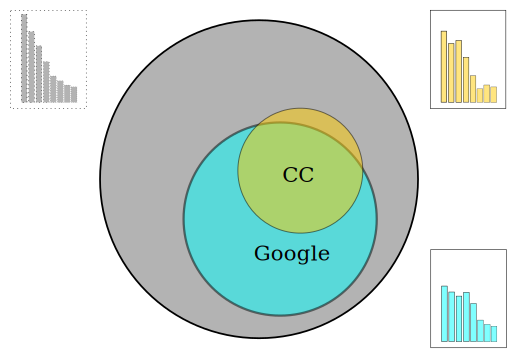
\includegraphics[width=\textwidth]{images/selection_bias}}

\vspace{.1cm}
\makebox[\textwidth][c]{\includegraphics[width=1.1\textwidth]{plots/plot_tld_comparison}}

\section{Public Suffix}
\vspace{.1cm}
\makebox[\textwidth][c]{\includegraphics[width=1.1\textwidth]{plots/plot_pub_suffixes_top10}}

\vspace{.1cm}
\makebox[\textwidth][c]{\includegraphics[width=1.1\textwidth]{plots/plot_pub_suffixes}}

\section{Mime-Type}
\vspace{.1cm}
\makebox[\textwidth][c]{\includegraphics[width=1.1\textwidth]{plots/plot_mime}}

\section{TLS}
\vspace{.1cm}
%\makebox[\textwidth][c]{\includegraphics[width=1.1\textwidth]{plots/plot_https}}

\section{Encoding}
\vspace{.1cm}
\makebox[\textwidth][c]{\includegraphics[width=1.1\textwidth]{plots/plot_charset}}

\section{Server}
\vspace{.1cm}
\makebox[\textwidth][c]{\includegraphics[width=1.1\textwidth]{plots/plot_server}}


\chapter{Textextraktion}

\centering{
    \includegraphics[trim=0 105px 0 0, clip=true, width=.9\textwidth]{images/guardian-website}
}

\scriptsize
\vspace{.1cm}
\url{http://www.theguardian.com/world/2013/jun/09/edward-snowden-nsa-whistleblower-surveillance}

\scriptsize
Edward Snowden: the whistleblower behind the NSA surveillance revelations $|$ US news $|$ The Guardian

\section{jWarcEx}

\begin{lstlisting}[breaklines=true]
Skip to main content

browse all sections close

Glenn Greenwald on security and liberty

Edward Snowden: the whistleblower behind the NSA surveillance revelations

The 29-year-old source behind the biggest intelligence leak in the NSA's history explains his motives, his uncertain future and why he never intended on hiding in the shadows

Q\&A with NSA whistleblower Edward Snowden: ``I do not expect to see home again''

Glenn Greenwald, Ewen MacAskill and Laura Poitras in Hong Kong

Tuesday 11 June 2013 09.00 EDT Last modified on Saturday 4 October 2014 10.54 EDT

Sorry, your browser is unable to play this video.

The individual responsible for one of the most significant leaks in US political history is Edward Snowden, a 29-year-old former technical assistant for the CIA and current employee of the defence contractor Booz Allen Hamilton. Snowden has been working at the National Security Agency for the last four years as an employee of various outside contractors, including Booz Allen and Dell.

The Guardian, after several days of interviews, is revealing his identity at his request. From the moment he decided to disclose numerous top-secret documents to the public, he was determined not to opt for the protection of anonymity. ``I have no intention of hiding who I am because I know I have done nothing wrong,'' he said.

(...)
\end{lstlisting}

\section{Mozilla Readability.js}

\begin{lstlisting}[breaklines=true]
Edward Snowden: the whistleblower behind the NSA surveillance revelations

Laura Poitras

The individual responsible for one of the most significant leaks in US political history is Edward Snowden, a 29-year-old former technical assistant for the CIA and current employee of the defence contractor Booz Allen Hamilton. Snowden has been working at the National Security Agency for the last four years as an employee of various outside contractors, including Booz Allen and Dell.

The Guardian, after several days of interviews, is revealing his identity at his request. From the moment he decided to disclose numerous top-secret documents to the public, he was determined not to opt for the protection of anonymity. ``I have no intention of hiding who I am because I know I have done nothing wrong,'' he said.

(...)
\end{lstlisting}

\section{Common Crawl}

\begin{lstlisting}[breaklines=true]
Lance Armstrong, Tour de France champ, retires | abc7.com

GO

Personalize your weather by entering a location.

Sorry, but the location you entered was not found. Please try again.

Sections

Traffic

Video

Los AngelesOrange CountyInland EmpireVentura CountyCalifornia

Home

Accuweather

Traffic

Video

Photos

Mobile Apps

Local News Los AngelesOrange CountyInland EmpireVentura CountyCalifornia

Map My News

Shows Live Well Network

Follow Us

BREAKING NEWS

(...)
\end{lstlisting}

\vspace{.2cm}
\url{http://abc7.com/archive/7962461}

\section{jWarcEx}

\begin{lstlisting}[breaklines=true]
Personalize your weather by entering a location.

Sorry, but the location you entered was not found. Please try again.

\vspace{.2cm}
Sections Traffic Video Los AngelesOrange CountyInland EmpireVentura CountyCalifornia

Home Accuweather Traffic Video Photos Mobile Apps

Los AngelesOrange CountyInland EmpireVentura CountyCalifornia

\quad BREAKING NEWS ABC shows live and on-demand -- Download the WATCH ABC app!

\vspace{.2cm}
Lance Armstrong, Tour de France champ, retires

Seven-time Tour de France champion Lance Armstrong is retiring. He ends his career amidst a federal doping investigation.

February 16, 2011 12:00:00 AM PST

Seven-time Tour de France champion Lance Armstrong said he's retiring from the professional cycling circuit, this time for good. The 39-year-old is calling it ``Retirement 2.0'' and is making it clear there is no reset button this time.

\vspace{.2cm}
He says he wants to spend more time with his children and dedicate himself even more to the fight against cancer with his "Livestrong" Foundation.

(...)
\end{lstlisting}

\vspace{.2cm}
\url{http://abc7.com/archive/7962461}


\end{document}
